\section{Introduction}
This work was presented at the European Congress on Digital Pathology 2019 and published as part of its proceedings ~\citep{carse2019active}.

\subsection{Active Learning for Medical Image Analysis}
Modern deep learning algorithms have been shown to improve performance for medical image analysis tasks such as classification, segmentation, and detection for different medical modalities including digital pathology. However, deep learning algorithms require large, annotated datasets to train models as these models learn a deep feature representation as well as a discriminative classifier. This requirement for data has been identified as a key challenge for using deep learning algorithms for digital pathology~\citep{tizhoosh2018artificial} and medical image analysis in general~\citep{litjens2017survey}. There are several approaches to tackling this problem including semi-supervised learning, weakly supervised learning, active learning, and combinations of these approaches. This work focuses on the use of active learning to aid in annotation collection for patch-based digital pathology.

Active learning is a type of machine learning that hypothesises that having a learning algorithm select the data that is used during training can reduce the amount of data needed for training~\citep{settles2012active}. Active learning is used within modern applications to reduce the quantity of data that needs to be annotated by selecting unannotated data to be annotated and added to the dataset used to train the model. By limiting the amount of data annotations needed can reduce annotation costs (which can be expensive when dealing with specialised data such as histopathology) and computation costs as the models can be trained with less data. In a pool-based scenario, the learning algorithm has access to a large pool of unannotated data. Over multiple iterations, the learning algorithm selects the most beneficial data from the pool to be annotated and added the training dataset, as shown in figure \ref{fig:pool_based_active_learning}.

\begin{figure}[h]
	\centering
	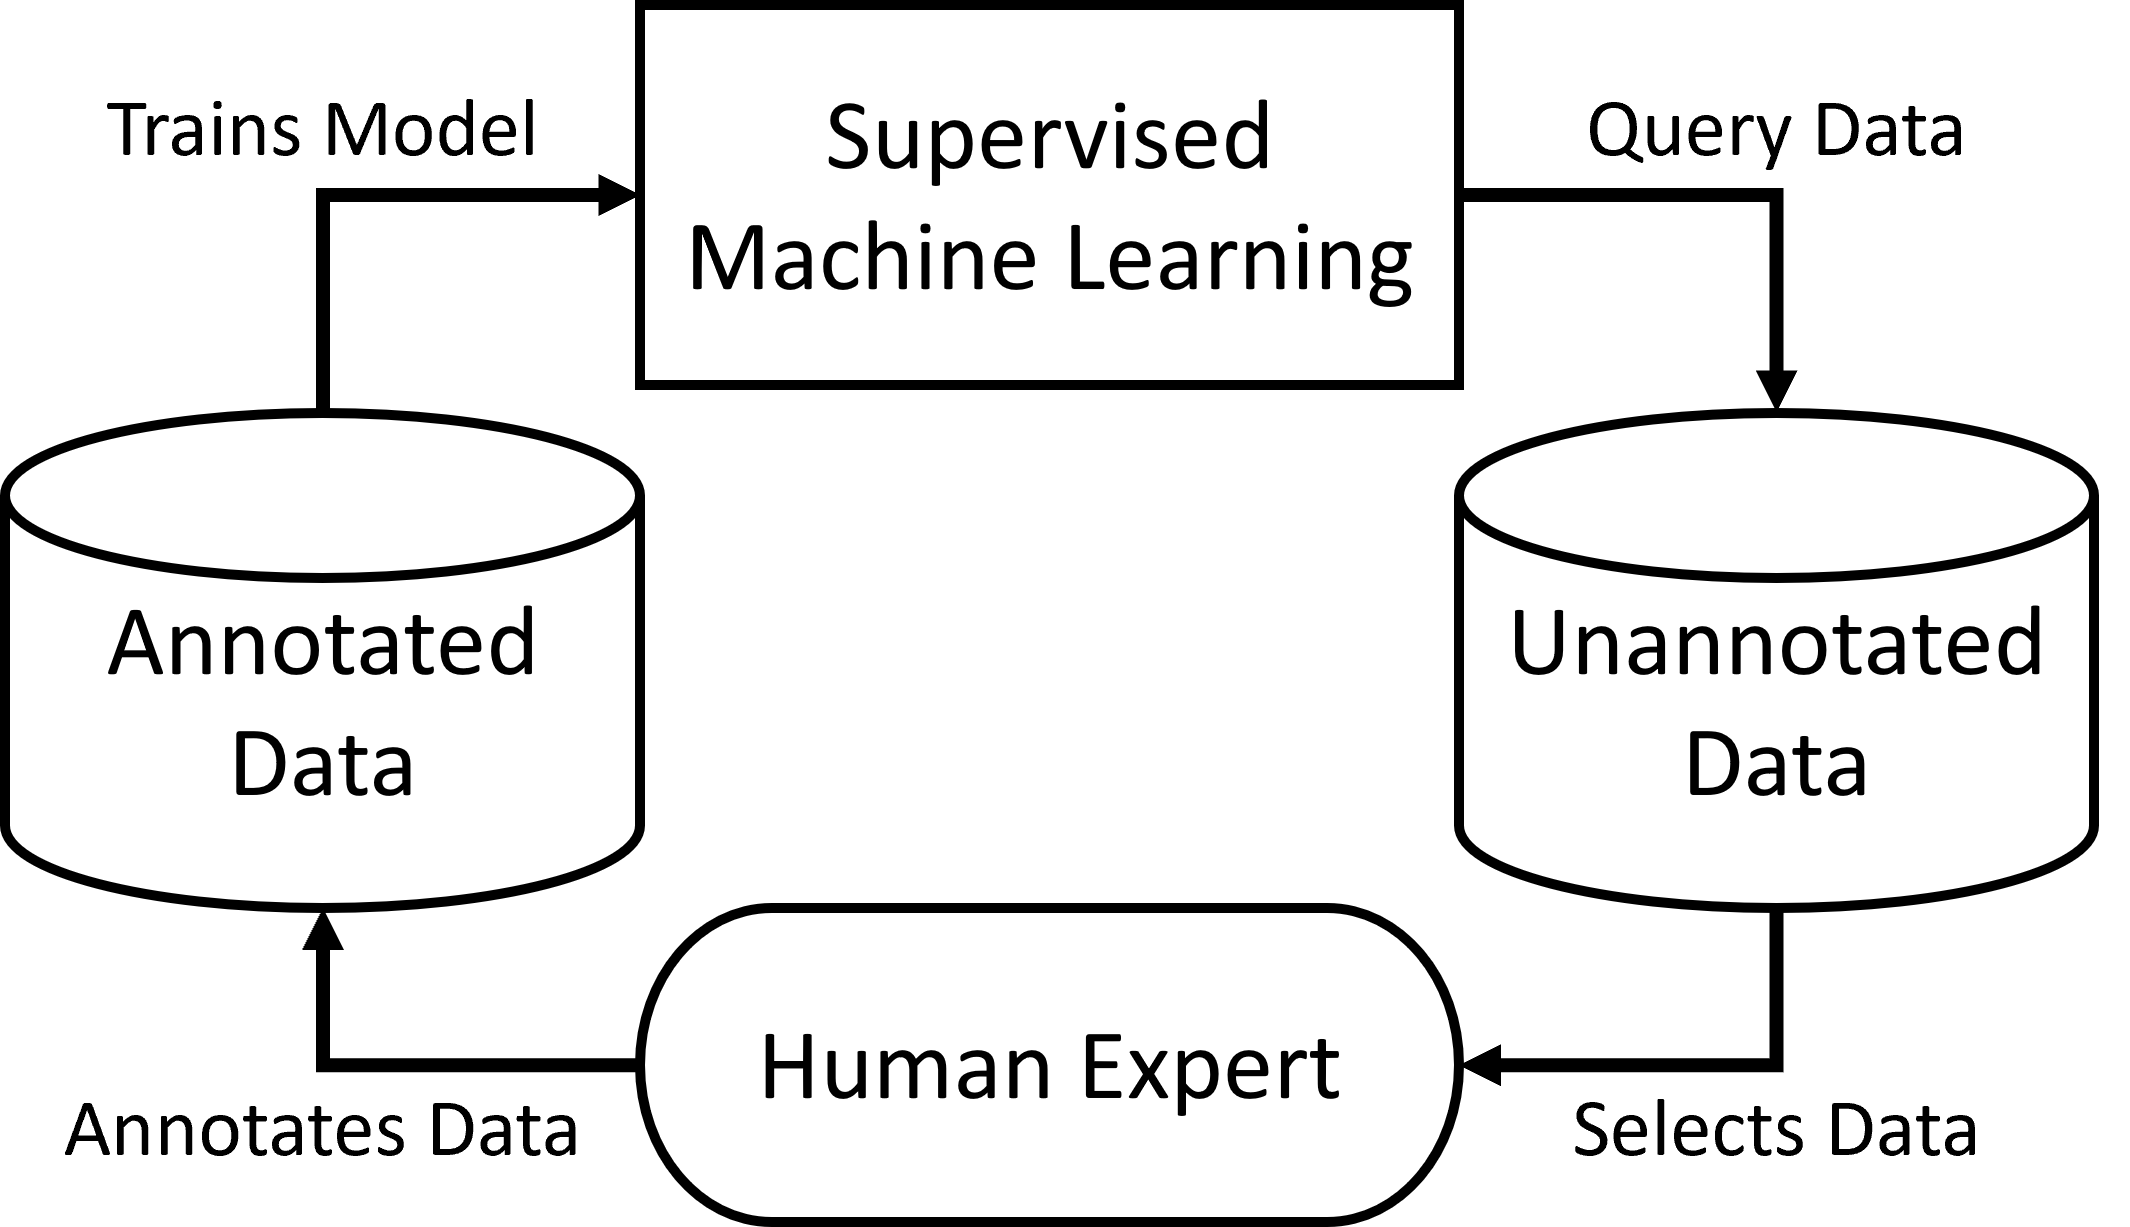
\includegraphics[width=0.75\textwidth]{images/active_learning.png}
	\caption{Pool-based active learning framework.}
	\label{fig:pool_based_active_learning}
\end{figure}

Active learning algorithms use query strategies to decide which data is to be selected for annotation. There are numerous query strategies available with the most popular methods being based on model uncertainty. Uncertainty sampling is a query strategy that focuses on selecting unannotated data that the model’s prediction is most uncertain about.

While these methods have been shown to perform well with many traditional learning algorithms, this is not the case when working with deep learning algorithms. There are several reasons for this, firstly, deep learning algorithms jointly learn feature representations and a classifier/regressor. Selecting only the difficult examples to train the model leads to the learnt features are not representative of the entire data distribution, decreasing the quality of the model~\citep{wang2016cost}. Secondly, traditional query strategies usually select a single data point, and it has been shown that deep learning algorithms perform better in an active learning environment with batch updates and so require a query strategy to select an optimal batch and not just a collection of the top-ranked points~\citep{sener2017active}. Thirdly, the softmax output from a classifier trained using deep learning algorithms does not represent the model’s uncertainty well, despite this the softmax output is still commonly used to represent uncertainty~\citep{gal2016dropout}.

\subsection{Deep Active Learning for Digital Pathology}
A standard approach for using learning algorithms for digital pathology is to use patches from larger images. This allows the images to be input to learning algorithms such as convolutional neural networks (CNNs) more efficiently and removes the necessity of annotating very large images. When using patch-based methods that use small patches, for tasks such as nuclei detection and classification, using active learning to select patches for annotation can be detrimental to annotation collection. This is due to small patches being time-consuming and tedious to annotate, small patches may also not include enough spatial context for accurate annotation.

To address these issues of using active learning for patch-based digital pathology, this work modifies the standard active learning framework to select regions for annotation that are built up of several patches to increase annotation throughput. This modified framework was evaluated with several active learning query strategies on a nuclei detection and classification task~\citep{sirinukunwattana2016locality}.



\section{Active Learning for Medical Images Review}
Active Learning for Medical Images Review

\subsection{Application of Active Learning for Medicine}
Application of Active Learning for Medicine

\subsection{Pool Based Active Learning Method}
Pool Based Active Learning Method 

\subsubsection{Traditional Machine Learning Query Strategies}
Traditional Machine Learning Query Strategies

\subsubsection{Deep Learning Query Strategies}
Deep Learning Query Strategies

\subsection{Active Learning for Annotation Efficiently}
Active Learning for Annotation Efficiently

\subsection{Annotator Efficient Active Learning for Histopathology}
Annotator Efficient Active Learning for Histopathology



\section{Annotator Efficient Active Learning for Histopathology}
Annotator Efficient Active Learning for Histopathology

\subsection{Problem Setting defined by Review}
Problem Setting defined by Review

\subsection{Region-Based Active Learning}
Patch-based methods are common within digital pathology and medical image analysis more generally. However, applying active learning to these methods can be tedious, especially in systems that use small patches. Small patches can be difficult to annotate in isolation. Even if their spatial visual context is provided to the annotator, continually having to reassess the context for each annotation can be inefficient and frustrating.  We propose a region-based alternative that requests annotations over larger regions containing multiple small patches. Working with larger regions eases the effort needed from the annotator and can lead to an improved annotation collection throughput. This alteration allows for a learning algorithm to be trained with the small patches and only treats the data as regions when querying the unannotated data.

\begin{algorithm}
	\caption{Region-based active learning}
	\label{alg:regionbased}
	\SetKwInOut{Input}{Input}
	\SetKwInOut{Output}{Output}
	\SetKwProg{RegionQueryStrategy}{RegionQueryStrategy}{}{}
	\Input{
		$\theta \gets$ trained model,\\
		$\delta \gets$ prediction algorithm,\\
		$S \gets$ active learning query strategy,\\
		$U \gets$ set of unannotated data,\\
		$A \gets$ set of annotated data
	}
	\Output{
		$U' \gets$ updated set of unannotated data,\\
		$A' \gets$ updated set of annotated data
	}
	\RegionQueryStrategy{$\theta, \delta, S, U, A$}
	{
		\ForEach{region $r$ in $U$}{
			$P \gets$ ExtractPatches($r$) \hfill extract patches from region\\
			$O \gets \theta(\delta, P)$ \hfill predictions on extracted patches\\
			$O' \gets$ Average($O$) \hfill average the patch predictions\\
			$Y \gets$ Append($Y, O'$) \hfill append region average to array\\
		}
		$n \gets S(Y)$ \hfill selects region from list\\
		$U' \gets$ Remove($U, n$) \hfill removes selection from unannotated set\\
		$A' \gets$ Append($A, n$) \hfill appends the selection to annotated set\\
		\Return{$U', A'$}
	}
\end{algorithm}

The proposed query strategy makes a simple modification to how an existing query strategy works. An overview of this can be seen in Algorithm \ref{alg:regionbased} where \(S\) is an existing query strategy. This algorithm is called at the end of each active iteration once a model has been trained on the currently available annotations. It extracts all the patches from each unannotated region and makes predictions on each patch. These predictions are then averaged to create a prediction for the overall region. Once all the regions have predictions, these predictions can be used within an active learning query strategy. An example of this would be using entropy uncertainty sampling where an uncertainty value for each region would be calculated and sampled. However, this approach can also be applied to more complex query strategies such as core-set sampling, by solving the K-centre problem for the region predictions rather than feature representations for individual data points.



\section{Active Learning Experiments}
This section details the datasets, training parameters, experimental setup, and results for the experiments with region-based active learning on a nuclei classification task from whole slide image patches. The code and full results used within this section can be found on the project GitHub repository\footnote{GitHub Repository: \url{github.com/jmcjacob/Patch-Active-Learning-Pathology}}.

\subsection{Dataset}
The publicly available CRCHistoPhenotypes~\citep{sirinukunwattana2016locality} dataset was used to evaluate region-based active learning as the dataset contained a large number of annotated nuclei from large patches extracted from whole slide images making it ideal for the use case for region based active learning. The dataset has also been used in several nuclei classification and detection studies and has also been used for active learning experiments~\citep{shao2018deep}. The dataset consists of 22,444 annotated nuclei from 100 500x500 non-overlapping patches from 10 whole slide H\&E images of colorectal adenocarcinomas from 9 different patients. Each nucleus has its coordinates and its corresponding classification (epithelial, inflammatory, fibroblast, and miscellaneous) annotated. There are 7,722 epithelial, 5,712 fibroblast, 6971 inflammatory and 2,039 miscellaneous annotated nuclei in the dataset. 2,500 images were produced by splitting the patches into 100x100 pixel regions. From these regions, each nucleus was extracted into a 30x30 patch that was used to train the CNN model. Augmentation was used during training by randomly applying Gaussian blurring and horizontal and vertical flipping.

\begin{figure}[t!]
	\centering
	\begin{subfigure}{0.3\textwidth}
		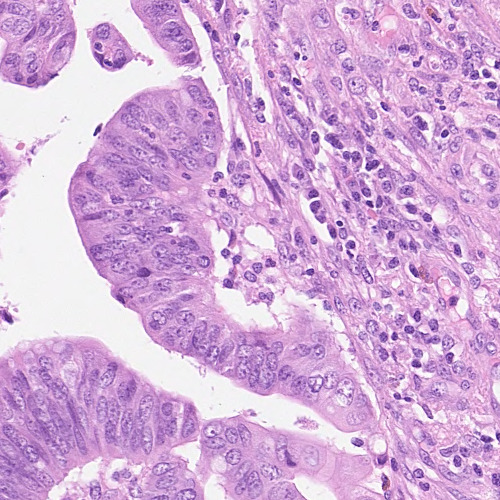
\includegraphics[width=\linewidth]{region1.jpg}
	\end{subfigure}
	\begin{subfigure}{0.3\textwidth}
		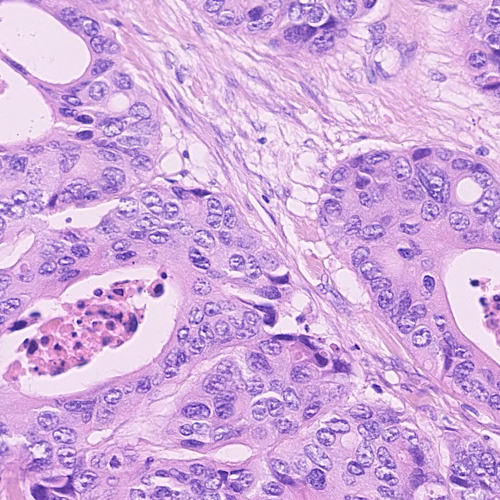
\includegraphics[width=\linewidth]{region2.jpg}
	\end{subfigure}
	\begin{subfigure}{0.3\textwidth}
		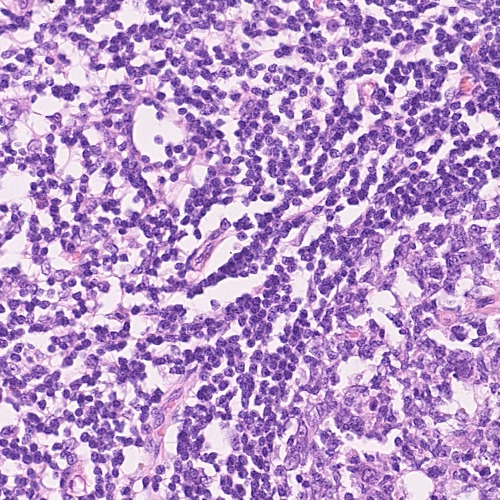
\includegraphics[width=\linewidth]{region3.jpg}
	\end{subfigure}
	\caption{Three example regions from the CRCHistoPhenotypes dataset~\cite{sirinukunwattana2016locality} with multiple nuclei that will be extracted into patches and augmented.}
	\label{fig:region_example}
\end{figure}

\subsection{Training Parameters}
This experiment used a simple CNN inspired by the architecture used in the nuclei classification benchmark for the CRCHistoPhenotypes dataset~\citep{sirinukunwattana2016locality}. It consisted of two convolutional layers, one with 36 4x4 filters and the other with 48 3x3 filters, both of which are followed by 2x2 max pooling layers. The convolutional layers were followed by two fully connected layers with 1200 neurons and 512 neurons respectively. This architecture is summarised in Table~\ref{tab:active_learning_cnn}. Each hidden layer used ReLU activation functions, and the two fully connected layers use dropout for regularisation~\citep{srivastava2014dropout} with a drop chance of 0.5. Dropout is used to train the model so the model can be used for Monte Carlo sampling after training.

\begin{table}[h]
	\caption{The Convolutional Neural Network architecture for nuclei classification used in the region-based active learning experiments.}
	\label{tab:active_learning_cnn}
	\centering
	\begin{tabular}{|c|c|c}
		\hline
		Type & \begin{tabular}[c]{@{}c@{}}Filter\\ Dimensions\end{tabular} & \multicolumn{1}{c|}{\begin{tabular}[c]{@{}c@{}}Input/Output\\ Dimensions\end{tabular}} \\ \hline
		I &  & \multicolumn{1}{c|}{30 x 30 x 3} \\ \hline
		C & 4 x 4 x 1 x 36 & \multicolumn{1}{c|}{26 x 26 x 36} \\ \hline
		M & 2 x 2 & \multicolumn{1}{c|}{12 x 12 x 36} \\ \hline
		C & 3 x 3 x 36 x 48 & \multicolumn{1}{c|}{10 x 10 x 48} \\ \hline
		M & 2 x 2 & \multicolumn{1}{c|}{5 x 5 x 48} \\ \hline
		F & 5 x 5 x 48 x 1200 & \multicolumn{1}{c|}{1 x 1200} \\ \hline
		F & 1 x 1 x 512 x 512 & \multicolumn{1}{c|}{1 x 512} \\ \hline
		F & 1 x 1 x 512 x 4 & \multicolumn{1}{c|}{1 x 4} \\ \hline
	\end{tabular}

\end{table}

During the active learning process, the training environment is constantly changing as the training data is increased. To keep up with this change the adaptive gradient decent algorithm Adadelta~\citep{zeiler2012adadelta} was chosen as it requires no manual tuning of the learning rate as it adapts to the gradients of the model. As the training environment is constantly changing and may have to deal with small quantities of annotated data models can easily overfit the training data, to avoid this early stopping is used. The method proposed by \cite{prechelt1998early} compares generalisation loss and training progression until it reaches a specified target $\frac{GL(t)}{P_k(t)} > \alpha$. Generalisation loss (Equation \ref{eq:generalization_loss}) is calculated by comparing the validation loss for each epoch \(L_{val}(t)\) against the minimum validation loss across all epochs. The training progression (Equation \ref{eq:generalization_loss}) value is calculated by analysing the training losses \(L_{tr}(t)\) over a batch of recent epochs of size \(k\).

\begin{equation}
	GL(t) = 100 \cdot \left ( \frac{L_{va}(t)}{\underset{t'\leq t}{min}L_{va}(t')} - 1 \right )
	\label{eq:generalization_loss}
\end{equation}
\begin{equation}
	P_k(t) = 1000 \cdot \left ( \frac{\sum_{t'=t-k+1}^{t}L_{tr}(t')}{k \cdot min^{t}_{t'=t-k+1}L_{tr}(t')} - 1\right )
	\label{eq:training_progression}
\end{equation}

\subsection{Experiment Setup}
Experiments testing the region-based active learning modification combined with a range of different query strategies. These query strategies included several basic methods used specifically to act as baselines compared to others built specifically for deep learning query algorithms. The baseline strategies chosen were random querying, least confident uncertainty, margin uncertainty and entropy uncertainty sampling. The deep learning-specific query strategies used were K-Centre sampling (using greedy approximation), core-set sampling~\citep{sener2017active} and Bayesian active learning by disagreement (BALD) using Monte Carlo dropout~\citep{gal2017deep}. These methods were chosen as they are state of the art for query strategies deep active learning methods, cost-effective active learning (CEAL)~\citep{wang2016cost} was considered for use in this study but due to its higher computational cost it was not used.

In each experiment, all the available data was initially treated as unannotated; two randomly selected regions were used to form the initial annotated training dataset. For each active iteration, two regions were selected from the unannotated pool of regions to be added to the training dataset, a randomly initialised model (using uniform Xavier initialisation~\citep{glorot2010understanding}) is then trained using the new dataset. This continued for 50 active iterations meaning that 102 regions out of 2,500 were used to form the final training set in each experiment. Each experimental setting was run five times with different seeds used to generate random elements (model weight initialisation and initial annotated patches).

\subsection{Results}
The query strategies were evaluated by testing the trained models after each active iteration on a single, unchanging test set. Table~\ref{tab:query_results} gives the test accuracy and cross-entropy loss after 50 iterations (averaged over five runs) for each of the tested query strategies. Notably, only K-Centre sampling achieved a higher average accuracy than a random sampling query strategy. The core-set sampling query strategy accuracy was very similar to that of random sampling. The other query strategies all performed worse than the random sampling baseline. Figures ~\ref{fig:active_learning_accuracy}, \ref{fig:active_learning_mean_class_accuracy} and \ref{fig:active_learning_loss} show the test accuracy, mean class accuracy and cross-entropy loss for the models trained with annotated data selected by each query strategy after each active iteration averaged over 5 runs. The figures also show the results of training a model with all the available regions annotated (1487 annotated training regions). For comparison, a fully supervised CNN trained on the entire dataset of annotated regions achieved an accuracy of 68.53\% and a cross-entropy loss of 1.111. Training using the K-Centre query strategy achieved an accuracy of 61.41\% and a cross-entropy loss of 1.137 using only 7\% of the annotated data.

\begin{table}
	\centering
	\caption{Test results for each query strategy after 50 active iterations.}
	\label{tab:query_results}
	\resizebox{\textwidth}{!}{%
		\begin{tabular}{c|ccccccc}
			\begin{tabular}[c]{@{}c@{}}Query\\ Strategy\end{tabular} & Random & \begin{tabular}[c]{@{}c@{}}Least \\ Confident\end{tabular} & Margin & Entropy & K-Centre & Core-Set & BALD \\ \hline
			Accuracy & 58.25 & 48.92 & 45.84 & 32.37 & 61.41 & 57.33 & 48.23 \\
			\begin{tabular}[c]{@{}c@{}}Mean Class \\ Accuracy\end{tabular} & 53.50 & 47.36 & 42.40 & 41.07 & 54.39 & 52.50 & 46.14 \\
			Loss & 1.154 & 1.243 & 1.268 & 1.39 & 1.123 & 1.157 & 1.247
		\end{tabular}%
	}
\end{table}

\begin{figure}
	\centering
	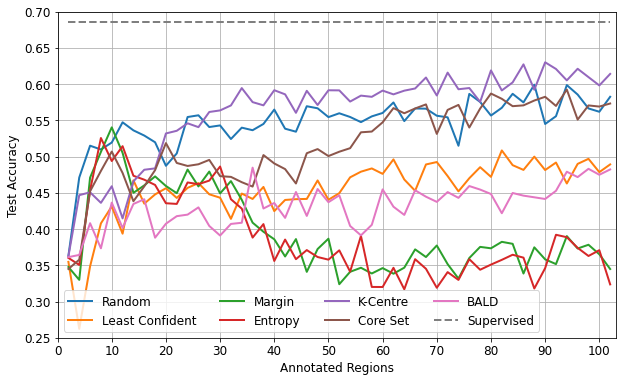
\includegraphics[width=\textwidth]{images/active_learning_accuracy.png}
	\caption{Average test accuracy of trained models with different amounts of annotated regions selected with query strategises.}
	\label{fig:active_learning_accuracy}
\end{figure}

\begin{figure}
	\centering
	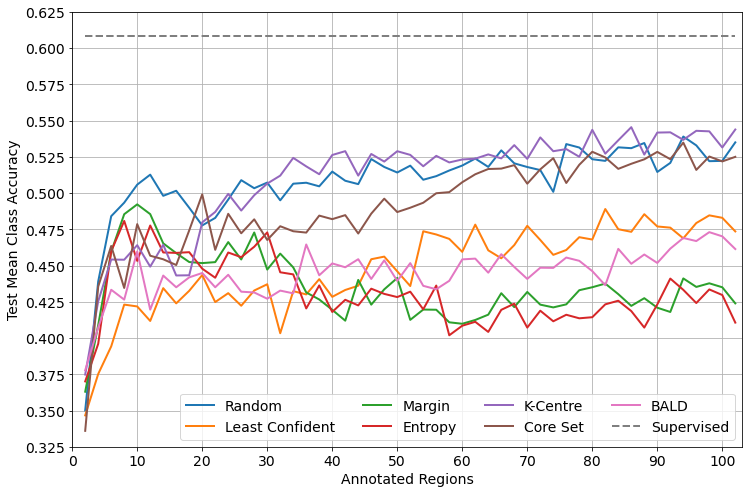
\includegraphics[width=\textwidth]{images/active_learning_mean_class_accuracy.png}
	\caption{Average test mean class accuracy of trained models with different amounts of annotated regions selected with query strategises.}
	\label{fig:active_learning_mean_class_accuracy}
\end{figure}

\begin{figure}
	\centering
	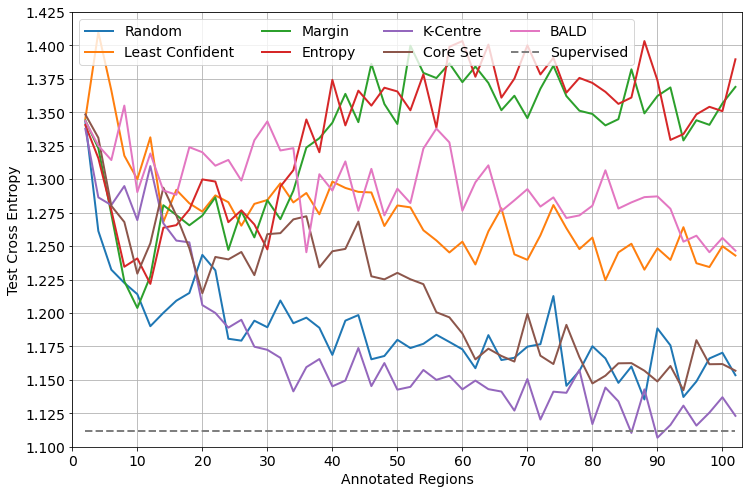
\includegraphics[width=\textwidth]{images/active_learning_loss.png}
	\caption{Average test loss of trained models with different amounts of annotated regions selected with query strategises.}
	\label{fig:active_learning_loss}
\end{figure}


\section{Conclusion}
This paper proposed a mechanism for applying deep active learning to patch-based systems with a specific focus on its application to nuclei classification. The results clearly showed that the traditional active learning query strategies performed poorly. Active learning methods tailored to deep CNNs are needed. Reducing annotation overheads and thus the cost of developing deep learning systems for digital pathology and medical image analysis can allow those with less access to resources to work on a range of problems. Methods such as active learning have great potential but further work is needed in order to achieve significant gains on tasks such as that investigated here. 
